\documentclass[a4paper,11pt,final]{article}
        \usepackage{fancyvrb, color, graphicx, hyperref, amsmath, url, textcomp}
        \usepackage{palatino}
        \usepackage[a4paper,text={16.5cm,25.2cm},centering]{geometry}

        %Set different options for xetex and luatex
        \usepackage{iftex}
        \ifxetex\usepackage{fontspec}\fi

        \ifluatex\usepackage{fontspec}\fi

        \hypersetup
        {   pdfauthor = {Pweave},
            pdftitle={Published from ctd.py},
            colorlinks=TRUE,
            linkcolor=black,
            citecolor=blue,
            urlcolor=blue
        }
        \setlength{\parindent}{0pt}
        \setlength{\parskip}{1.2ex}
        % fix for pandoc 1.14
        \providecommand{\tightlist}{%
            \setlength{\itemsep}{0pt}\setlength{\parskip}{0pt}}
        
\makeatletter
\def\PY@reset{\let\PY@it=\relax \let\PY@bf=\relax%
    \let\PY@ul=\relax \let\PY@tc=\relax%
    \let\PY@bc=\relax \let\PY@ff=\relax}
\def\PY@tok#1{\csname PY@tok@#1\endcsname}
\def\PY@toks#1+{\ifx\relax#1\empty\else%
    \PY@tok{#1}\expandafter\PY@toks\fi}
\def\PY@do#1{\PY@bc{\PY@tc{\PY@ul{%
    \PY@it{\PY@bf{\PY@ff{#1}}}}}}}
\def\PY#1#2{\PY@reset\PY@toks#1+\relax+\PY@do{#2}}

\expandafter\def\csname PY@tok@k\endcsname{\let\PY@bf=\textbf\def\PY@tc##1{\textcolor[rgb]{0.00,0.50,0.00}{##1}}}
\expandafter\def\csname PY@tok@kc\endcsname{\let\PY@bf=\textbf\def\PY@tc##1{\textcolor[rgb]{0.00,0.50,0.00}{##1}}}
\expandafter\def\csname PY@tok@kp\endcsname{\def\PY@tc##1{\textcolor[rgb]{0.00,0.50,0.00}{##1}}}
\expandafter\def\csname PY@tok@sr\endcsname{\def\PY@tc##1{\textcolor[rgb]{0.73,0.40,0.53}{##1}}}
\expandafter\def\csname PY@tok@se\endcsname{\let\PY@bf=\textbf\def\PY@tc##1{\textcolor[rgb]{0.73,0.40,0.13}{##1}}}
\expandafter\def\csname PY@tok@ss\endcsname{\def\PY@tc##1{\textcolor[rgb]{0.10,0.09,0.49}{##1}}}
\expandafter\def\csname PY@tok@bp\endcsname{\def\PY@tc##1{\textcolor[rgb]{0.00,0.50,0.00}{##1}}}
\expandafter\def\csname PY@tok@gh\endcsname{\let\PY@bf=\textbf\def\PY@tc##1{\textcolor[rgb]{0.00,0.00,0.50}{##1}}}
\expandafter\def\csname PY@tok@nc\endcsname{\let\PY@bf=\textbf\def\PY@tc##1{\textcolor[rgb]{0.00,0.00,1.00}{##1}}}
\expandafter\def\csname PY@tok@si\endcsname{\let\PY@bf=\textbf\def\PY@tc##1{\textcolor[rgb]{0.73,0.40,0.53}{##1}}}
\expandafter\def\csname PY@tok@sh\endcsname{\def\PY@tc##1{\textcolor[rgb]{0.73,0.13,0.13}{##1}}}
\expandafter\def\csname PY@tok@c1\endcsname{\let\PY@it=\textit\def\PY@tc##1{\textcolor[rgb]{0.25,0.50,0.50}{##1}}}
\expandafter\def\csname PY@tok@na\endcsname{\def\PY@tc##1{\textcolor[rgb]{0.49,0.56,0.16}{##1}}}
\expandafter\def\csname PY@tok@gs\endcsname{\let\PY@bf=\textbf}
\expandafter\def\csname PY@tok@nt\endcsname{\let\PY@bf=\textbf\def\PY@tc##1{\textcolor[rgb]{0.00,0.50,0.00}{##1}}}
\expandafter\def\csname PY@tok@nf\endcsname{\def\PY@tc##1{\textcolor[rgb]{0.00,0.00,1.00}{##1}}}
\expandafter\def\csname PY@tok@s\endcsname{\def\PY@tc##1{\textcolor[rgb]{0.73,0.13,0.13}{##1}}}
\expandafter\def\csname PY@tok@c\endcsname{\let\PY@it=\textit\def\PY@tc##1{\textcolor[rgb]{0.25,0.50,0.50}{##1}}}
\expandafter\def\csname PY@tok@mf\endcsname{\def\PY@tc##1{\textcolor[rgb]{0.40,0.40,0.40}{##1}}}
\expandafter\def\csname PY@tok@gu\endcsname{\let\PY@bf=\textbf\def\PY@tc##1{\textcolor[rgb]{0.50,0.00,0.50}{##1}}}
\expandafter\def\csname PY@tok@kt\endcsname{\def\PY@tc##1{\textcolor[rgb]{0.69,0.00,0.25}{##1}}}
\expandafter\def\csname PY@tok@ni\endcsname{\let\PY@bf=\textbf\def\PY@tc##1{\textcolor[rgb]{0.60,0.60,0.60}{##1}}}
\expandafter\def\csname PY@tok@gp\endcsname{\let\PY@bf=\textbf\def\PY@tc##1{\textcolor[rgb]{0.00,0.00,0.50}{##1}}}
\expandafter\def\csname PY@tok@mi\endcsname{\def\PY@tc##1{\textcolor[rgb]{0.40,0.40,0.40}{##1}}}
\expandafter\def\csname PY@tok@kn\endcsname{\let\PY@bf=\textbf\def\PY@tc##1{\textcolor[rgb]{0.00,0.50,0.00}{##1}}}
\expandafter\def\csname PY@tok@vg\endcsname{\def\PY@tc##1{\textcolor[rgb]{0.10,0.09,0.49}{##1}}}
\expandafter\def\csname PY@tok@mo\endcsname{\def\PY@tc##1{\textcolor[rgb]{0.40,0.40,0.40}{##1}}}
\expandafter\def\csname PY@tok@mh\endcsname{\def\PY@tc##1{\textcolor[rgb]{0.40,0.40,0.40}{##1}}}
\expandafter\def\csname PY@tok@o\endcsname{\def\PY@tc##1{\textcolor[rgb]{0.40,0.40,0.40}{##1}}}
\expandafter\def\csname PY@tok@il\endcsname{\def\PY@tc##1{\textcolor[rgb]{0.40,0.40,0.40}{##1}}}
\expandafter\def\csname PY@tok@ne\endcsname{\let\PY@bf=\textbf\def\PY@tc##1{\textcolor[rgb]{0.82,0.25,0.23}{##1}}}
\expandafter\def\csname PY@tok@sd\endcsname{\let\PY@it=\textit\def\PY@tc##1{\textcolor[rgb]{0.73,0.13,0.13}{##1}}}
\expandafter\def\csname PY@tok@gi\endcsname{\def\PY@tc##1{\textcolor[rgb]{0.00,0.63,0.00}{##1}}}
\expandafter\def\csname PY@tok@err\endcsname{\def\PY@bc##1{\setlength{\fboxsep}{0pt}\fcolorbox[rgb]{1.00,0.00,0.00}{1,1,1}{\strut ##1}}}
\expandafter\def\csname PY@tok@kd\endcsname{\let\PY@bf=\textbf\def\PY@tc##1{\textcolor[rgb]{0.00,0.50,0.00}{##1}}}
\expandafter\def\csname PY@tok@nb\endcsname{\def\PY@tc##1{\textcolor[rgb]{0.00,0.50,0.00}{##1}}}
\expandafter\def\csname PY@tok@nv\endcsname{\def\PY@tc##1{\textcolor[rgb]{0.10,0.09,0.49}{##1}}}
\expandafter\def\csname PY@tok@s1\endcsname{\def\PY@tc##1{\textcolor[rgb]{0.73,0.13,0.13}{##1}}}
\expandafter\def\csname PY@tok@kr\endcsname{\let\PY@bf=\textbf\def\PY@tc##1{\textcolor[rgb]{0.00,0.50,0.00}{##1}}}
\expandafter\def\csname PY@tok@sx\endcsname{\def\PY@tc##1{\textcolor[rgb]{0.00,0.50,0.00}{##1}}}
\expandafter\def\csname PY@tok@ch\endcsname{\let\PY@it=\textit\def\PY@tc##1{\textcolor[rgb]{0.25,0.50,0.50}{##1}}}
\expandafter\def\csname PY@tok@gd\endcsname{\def\PY@tc##1{\textcolor[rgb]{0.63,0.00,0.00}{##1}}}
\expandafter\def\csname PY@tok@go\endcsname{\def\PY@tc##1{\textcolor[rgb]{0.53,0.53,0.53}{##1}}}
\expandafter\def\csname PY@tok@sc\endcsname{\def\PY@tc##1{\textcolor[rgb]{0.73,0.13,0.13}{##1}}}
\expandafter\def\csname PY@tok@no\endcsname{\def\PY@tc##1{\textcolor[rgb]{0.53,0.00,0.00}{##1}}}
\expandafter\def\csname PY@tok@cs\endcsname{\let\PY@it=\textit\def\PY@tc##1{\textcolor[rgb]{0.25,0.50,0.50}{##1}}}
\expandafter\def\csname PY@tok@vc\endcsname{\def\PY@tc##1{\textcolor[rgb]{0.10,0.09,0.49}{##1}}}
\expandafter\def\csname PY@tok@w\endcsname{\def\PY@tc##1{\textcolor[rgb]{0.73,0.73,0.73}{##1}}}
\expandafter\def\csname PY@tok@nl\endcsname{\def\PY@tc##1{\textcolor[rgb]{0.63,0.63,0.00}{##1}}}
\expandafter\def\csname PY@tok@cp\endcsname{\def\PY@tc##1{\textcolor[rgb]{0.74,0.48,0.00}{##1}}}
\expandafter\def\csname PY@tok@s2\endcsname{\def\PY@tc##1{\textcolor[rgb]{0.73,0.13,0.13}{##1}}}
\expandafter\def\csname PY@tok@m\endcsname{\def\PY@tc##1{\textcolor[rgb]{0.40,0.40,0.40}{##1}}}
\expandafter\def\csname PY@tok@cpf\endcsname{\let\PY@it=\textit\def\PY@tc##1{\textcolor[rgb]{0.25,0.50,0.50}{##1}}}
\expandafter\def\csname PY@tok@gr\endcsname{\def\PY@tc##1{\textcolor[rgb]{1.00,0.00,0.00}{##1}}}
\expandafter\def\csname PY@tok@nn\endcsname{\let\PY@bf=\textbf\def\PY@tc##1{\textcolor[rgb]{0.00,0.00,1.00}{##1}}}
\expandafter\def\csname PY@tok@nd\endcsname{\def\PY@tc##1{\textcolor[rgb]{0.67,0.13,1.00}{##1}}}
\expandafter\def\csname PY@tok@ow\endcsname{\let\PY@bf=\textbf\def\PY@tc##1{\textcolor[rgb]{0.67,0.13,1.00}{##1}}}
\expandafter\def\csname PY@tok@ge\endcsname{\let\PY@it=\textit}
\expandafter\def\csname PY@tok@cm\endcsname{\let\PY@it=\textit\def\PY@tc##1{\textcolor[rgb]{0.25,0.50,0.50}{##1}}}
\expandafter\def\csname PY@tok@gt\endcsname{\def\PY@tc##1{\textcolor[rgb]{0.00,0.27,0.87}{##1}}}
\expandafter\def\csname PY@tok@vi\endcsname{\def\PY@tc##1{\textcolor[rgb]{0.10,0.09,0.49}{##1}}}
\expandafter\def\csname PY@tok@sb\endcsname{\def\PY@tc##1{\textcolor[rgb]{0.73,0.13,0.13}{##1}}}
\expandafter\def\csname PY@tok@mb\endcsname{\def\PY@tc##1{\textcolor[rgb]{0.40,0.40,0.40}{##1}}}

\def\PYZbs{\char`\\}
\def\PYZus{\char`\_}
\def\PYZob{\char`\{}
\def\PYZcb{\char`\}}
\def\PYZca{\char`\^}
\def\PYZam{\char`\&}
\def\PYZlt{\char`\<}
\def\PYZgt{\char`\>}
\def\PYZsh{\char`\#}
\def\PYZpc{\char`\%}
\def\PYZdl{\char`\$}
\def\PYZhy{\char`\-}
\def\PYZsq{\char`\'}
\def\PYZdq{\char`\"}
\def\PYZti{\char`\~}
% for compatibility with earlier versions
\def\PYZat{@}
\def\PYZlb{[}
\def\PYZrb{]}
\makeatother

        
\begin{document}
\begin{Verbatim}[commandchars=\\\{\},frame=single,fontsize=\small, xleftmargin=0.5em]
\PY{c+c1}{\PYZsh{} coding: utf\PYZhy{}8}
\end{Verbatim}

\section{Exemplo: manipulação de NaNs e limpeza de
dados}\label{exemplo-manipulauxe7uxe3o-de-nans-e-limpeza-de-dados}

Neste exemplo, usaremos um arquivo com muitos dados ausentes
(representados por NaNs) para explorar o conceito de \emph{filtros}.
Além disso, vamos fazer um gráfico simples para representar os dados.
Para isso, vamos usar duas bibliotecas importantes: Pandas (que já
mencionamos) e matplotlib.

\begin{Verbatim}[commandchars=\\\{\},frame=single,fontsize=\small, xleftmargin=0.5em]
\PY{k+kn}{import} \PY{n+nn}{pandas} \PY{k+kn}{as} \PY{n+nn}{pd}
\end{Verbatim}

Primeiramente, vamos ler o arquivo usando tabs como separadores.

\begin{Verbatim}[commandchars=\\\{\},frame=single,fontsize=\small, xleftmargin=0.5em]
\PY{n}{dados} \PY{o}{=} \PY{n}{pd}\PY{o}{.}\PY{n}{read\PYZus{}csv}\PY{p}{(}\PY{l+s+s1}{\PYZsq{}}\PY{l+s+s1}{data\PYZus{}from\PYZus{}odv\PYZus{}data\PYZus{}carbon\PYZhy{}}
\PY{n}{sse\PYZus{}after\PYZus{}correction\PYZus{}spikes\PYZus{}v3\PYZus{}O2\PYZus{}corr}\PY{o}{.}\PY{n}{txt}\PY{l+s+s1}{\PYZsq{}}\PY{l+s+s1}{, sep = }\PY{l+s+s1}{\PYZsq{}}\PYZbs{}\PY{n}{t}\PY{l+s+s1}{\PYZsq{}}\PY{l+s+s1}{,}
\PY{n}{lineterminator}\PY{o}{=}\PY{l+s+s1}{\PYZsq{}}\PY{l+s+se}{\PYZbs{}n}\PY{l+s+s1}{\PYZsq{}}\PY{p}{)}
\PY{k}{print}\PY{p}{(}\PY{n}{dados}\PY{p}{)}
\end{Verbatim}
\begin{Verbatim}[commandchars=\\\{\},frame=leftline,fontsize=\small, xleftmargin=0.5em]
            Cruise Station Type mon/day/yr  hh:mm  Longitude
[degrees\PYZus{}east]  \PYZbs{}
0      NHoCruzeiro       5    C  12/6/2010  23:22
308.4600
1              NaN     NaN  NaN        NaN    NaN
NaN
2              NaN     NaN  NaN        NaN    NaN
NaN
3              NaN     NaN  NaN        NaN    NaN
NaN
4              NaN     NaN  NaN        NaN    NaN
NaN
5              NaN     NaN  NaN        NaN    NaN
NaN
6              NaN     NaN  NaN        NaN    NaN
NaN
7              NaN     NaN  NaN        NaN    NaN
NaN
8              NaN     NaN  NaN        NaN    NaN
NaN
9              NaN     NaN  NaN        NaN    NaN
NaN
10             NaN     NaN  NaN        NaN    NaN
NaN
11             NaN     NaN  NaN        NaN    NaN
NaN
12             NaN     NaN  NaN        NaN    NaN
NaN
13             NaN     NaN  NaN        NaN    NaN
NaN
14             NaN     NaN  NaN        NaN    NaN
NaN
15             NaN     NaN  NaN        NaN    NaN
NaN
16             NaN     NaN  NaN        NaN    NaN
NaN
17             NaN     NaN  NaN        NaN    NaN
NaN
18             NaN     NaN  NaN        NaN    NaN
NaN
19             NaN     NaN  NaN        NaN    NaN
NaN
20             NaN     NaN  NaN        NaN    NaN
NaN
21             NaN     NaN  NaN        NaN    NaN
NaN
22             NaN     NaN  NaN        NaN    NaN
NaN
23             NaN     NaN  NaN        NaN    NaN
NaN
24             NaN     NaN  NaN        NaN    NaN
NaN
25             NaN     NaN  NaN        NaN    NaN
NaN
26             NaN     NaN  NaN        NaN    NaN
NaN
27             NaN     NaN  NaN        NaN    NaN
NaN
28             NaN     NaN  NaN        NaN    NaN
NaN
29             NaN     NaN  NaN        NaN    NaN
NaN
...            ...     ...  ...        ...    ...
...
57652          NaN     NaN  NaN        NaN    NaN
NaN
57653          NaN     NaN  NaN        NaN    NaN
NaN
57654          NaN     NaN  NaN        NaN    NaN
NaN
57655          NaN     NaN  NaN        NaN    NaN
NaN
57656          NaN     NaN  NaN        NaN    NaN
NaN
57657          NaN     NaN  NaN        NaN    NaN
NaN
57658          NaN     NaN  NaN        NaN    NaN
NaN
57659          NaN     NaN  NaN        NaN    NaN
NaN
57660          NaN     NaN  NaN        NaN    NaN
NaN
57661          NaN     NaN  NaN        NaN    NaN
NaN
57662          NaN     NaN  NaN        NaN    NaN
NaN
57663  NHoCruzeiro    080e    B   1/7/2011   0:06
319.0342
57664          NaN     NaN  NaN        NaN    NaN
NaN
57665          NaN     NaN  NaN        NaN    NaN
NaN
57666          NaN     NaN  NaN        NaN    NaN
NaN
57667          NaN     NaN  NaN        NaN    NaN
NaN
57668          NaN     NaN  NaN        NaN    NaN
NaN
57669          NaN     NaN  NaN        NaN    NaN
NaN
57670          NaN     NaN  NaN        NaN    NaN
NaN
57671          NaN     NaN  NaN        NaN    NaN
NaN
57672          NaN     NaN  NaN        NaN    NaN
NaN
57673          NaN     NaN  NaN        NaN    NaN
NaN
57674          NaN     NaN  NaN        NaN    NaN
NaN
57675          NaN     NaN  NaN        NaN    NaN
NaN
57676          NaN     NaN  NaN        NaN    NaN
NaN
57677          NaN     NaN  NaN        NaN    NaN
NaN
57678          NaN     NaN  NaN        NaN    NaN
NaN
57679          NaN     NaN  NaN        NaN    NaN
NaN
57680          NaN     NaN  NaN        NaN    NaN
NaN
57681          NaN     NaN  NaN        NaN    NaN
NaN

       Latitude [degrees\PYZus{}north]  Bot. Depth [m]  Cast  QF       ...
\PYZbs{}
0                       \PYZhy{}34.384          1052.0     1   1       ...
1                           NaN             NaN     1   1       ...
2                           NaN             NaN     1   1       ...
3                           NaN             NaN     1   1       ...
4                           NaN             NaN     1   1       ...
5                           NaN             NaN     1   1       ...
6                           NaN             NaN     1   1       ...
7                           NaN             NaN     1   1       ...
8                           NaN             NaN     1   1       ...
9                           NaN             NaN     1   1       ...
10                          NaN             NaN     1   1       ...
11                          NaN             NaN     1   1       ...
12                          NaN             NaN     1   1       ...
13                          NaN             NaN     1   1       ...
14                          NaN             NaN     1   1       ...
15                          NaN             NaN     1   1       ...
16                          NaN             NaN     1   1       ...
17                          NaN             NaN     1   1       ...
18                          NaN             NaN     1   1       ...
19                          NaN             NaN     1   1       ...
20                          NaN             NaN     1   1       ...
21                          NaN             NaN     1   1       ...
22                          NaN             NaN     1   1       ...
23                          NaN             NaN     1   1       ...
24                          NaN             NaN     1   1       ...
25                          NaN             NaN     1   1       ...
26                          NaN             NaN     1   1       ...
27                          NaN             NaN     1   1       ...
28                          NaN             NaN     1   1       ...
29                          NaN             NaN     1   1       ...
...                         ...             ...   ...  ..       ...
57652                       NaN             NaN     1   1       ...
57653                       NaN             NaN     1   1       ...
57654                       NaN             NaN     1   1       ...
57655                       NaN             NaN     1   1       ...
57656                       NaN             NaN     1   1       ...
57657                       NaN             NaN     1   1       ...
57658                       NaN             NaN     1   1       ...
57659                       NaN             NaN     1   1       ...
57660                       NaN             NaN     1   1       ...
57661                       NaN             NaN     1   1       ...
57662                       NaN             NaN     1   1       ...
57663                   \PYZhy{}22.119            24.0     1   1       ...
57664                       NaN             NaN     1   1       ...
57665                       NaN             NaN     1   1       ...
57666                       NaN             NaN     1   1       ...
57667                       NaN             NaN     1   1       ...
57668                       NaN             NaN     1   1       ...
57669                       NaN             NaN     1   1       ...
57670                       NaN             NaN     1   1       ...
57671                       NaN             NaN     1   1       ...
57672                       NaN             NaN     1   1       ...
57673                       NaN             NaN     1   1       ...
57674                       NaN             NaN     1   1       ...
57675                       NaN             NaN     1   1       ...
57676                       NaN             NaN     1   1       ...
57677                       NaN             NaN     1   1       ...
57678                       NaN             NaN     1   1       ...
57679                       NaN             NaN     1   1       ...
57680                       NaN             NaN     1   1       ...
57681                       NaN             NaN     1   1       ...

       QF.19  Oxygen [ml l]  QF.20  Num Scan per bin  QF.21  flag
QF.22  \PYZbs{}
0          1           5.07      1                33      1   NaN
1
1          1           5.09      1                42      1   NaN
1
2          1           5.18      1                46      1   NaN
1
3          1           5.23      1                36      1   NaN
1
4          1           5.18      1                26      1   NaN
1
5          1           5.27      1                28      1   NaN
1
6          1           5.23      1                55      1   NaN
1
7          1           5.18      1                27      1   NaN
1
8          1           5.14      1                53      1   NaN
1
9          1           5.09      1                44      1   NaN
1
10         1           5.17      1                48      1   NaN
1
11         1           5.20      1                53      1   NaN
1
12         1           5.15      1                47      1   NaN
1
13         1           5.16      1                43      1   NaN
1
14         1           5.14      1                53      1   NaN
1
15         1           5.10      1                59      1   NaN
1
16         1           5.08      1                59      1   NaN
1
17         1           5.02      1                42      1   NaN
1
18         1           5.09      1                60      1   NaN
1
19         1           5.12      1                41      1   NaN
1
20         1           5.07      1                34      1   NaN
1
21         1           5.03      1                49      1   NaN
1
22         1           5.09      1                44      1   NaN
1
23         1           5.04      1                22      1   NaN
1
24         1           5.04      1                21      1   NaN
1
25         1           5.06      1                24      1   NaN
1
26         1           5.08      1                24      1   NaN
1
27         1           5.02      1                33      1   NaN
1
28         1           5.02      1                46      1   NaN
1
29         1           4.89      1                22      1   NaN
1
...      ...            ...    ...               ...    ...   ...
...
57652      1           4.53      1                46      1   NaN
1
57653      1           4.53      1                45      1   NaN
1
57654      1           4.51      1                28      1   NaN
1
57655      1           4.50      1                28      1   NaN
1
57656      1           4.50      1                57      1   NaN
1
57657      1           4.47      1                33      1   NaN
1
57658      1           4.38      1                31      1   NaN
1
57659      1           4.53      1                29      1   NaN
1
57660      1           4.60      1                60      1   NaN
1
57661      1           4.69      1                40      1   NaN
1
57662      1           4.72      1                35      1   NaN
1
57663      1           4.70      1                35      1   NaN
1
57664      1           4.63      1                24      1   NaN
1
57665      1           4.53      1                18      1   NaN
1
57666      1           4.26      1                19      1   NaN
1
57667      1           4.19      1                26      1   NaN
1
57668      1           4.37      1                34      1   NaN
1
57669      1           4.48      1                28      1   NaN
1
57670      1           4.56      1                51      1   NaN
1
57671      1           4.52      1                74      1   NaN
1
57672      1           4.41      1                54      1   NaN
1
57673      1           4.42      1                38      1   NaN
1
57674      1           4.41      1                46      1   NaN
1
57675      1           4.40      1                38      1   NaN
1
57676      1           4.41      1                81      1   NaN
1
57677      1           4.42      1                16      1   NaN
1
57678      1           4.48      1                22      1   NaN
1
57679      1           4.52      1                21      1   NaN
1
57680      1           4.55      1                25      1   NaN
1
57681      1           4.58      1                40      1   NaN
1

       Section Longitude:DOUBLE  QF.23  QV:ODV:SAMPLE\PYZbs{}r
0                           NaN      1                1
1                           NaN      1                1
2                           NaN      1                1
3                           NaN      1                1
4                           NaN      1                1
5                           NaN      1                1
6                           NaN      1                1
7                           NaN      1                1
8                           NaN      1                1
9                           NaN      1                1
10                          NaN      1                1
11                          NaN      1                1
12                          NaN      1                1
13                          NaN      1                1
14                          NaN      1                1
15                          NaN      1                1
16                          NaN      1                1
17                          NaN      1                1
18                          NaN      1                1
19                          NaN      1                1
20                          NaN      1                1
21                          NaN      1                1
22                          NaN      1                1
23                          NaN      1                1
24                          NaN      1                1
25                          NaN      1                1
26                          NaN      1                1
27                          NaN      1                1
28                          NaN      1                1
29                          NaN      1                1
...                         ...    ...              ...
57652                       NaN      1                1
57653                       NaN      1                1
57654                       NaN      1                1
57655                       NaN      1                1
57656                       NaN      1                1
57657                       NaN      1                1
57658                       NaN      1                1
57659                       NaN      1                1
57660                       NaN      1                1
57661                       NaN      1                1
57662                       NaN      1                1
57663                       NaN      1                1
57664                       NaN      1                1
57665                       NaN      1                1
57666                       NaN      1                1
57667                       NaN      1                1
57668                       NaN      1                1
57669                       NaN      1                1
57670                       NaN      1                1
57671                       NaN      1                1
57672                       NaN      1                1
57673                       NaN      1                1
57674                       NaN      1                1
57675                       NaN      1                1
57676                       NaN      1                1
57677                       NaN      1                1
57678                       NaN      1                1
57679                       NaN      1                1
57680                       NaN      1                1
57681                       NaN      1                1

[57682 rows x 57 columns]
\end{Verbatim}

Agora, vamos tentar identificar de quantas estações temos dados
disponíveis.

\begin{Verbatim}[commandchars=\\\{\},frame=single,fontsize=\small, xleftmargin=0.5em]
\PY{k}{print}\PY{p}{(}\PY{n}{dados}\PY{o}{.}\PY{n}{Station}\PY{o}{.}\PY{n}{head}\PY{p}{)}
\end{Verbatim}
\begin{Verbatim}[commandchars=\\\{\},frame=leftline,fontsize=\small, xleftmargin=0.5em]
\PYZlt{}bound method NDFrame.head of 0           5
1         NaN
2         NaN
3         NaN
4         NaN
5         NaN
6         NaN
7         NaN
8         NaN
9         NaN
10        NaN
11        NaN
12        NaN
13        NaN
14        NaN
15        NaN
16        NaN
17        NaN
18        NaN
19        NaN
20        NaN
21        NaN
22        NaN
23        NaN
24        NaN
25        NaN
26        NaN
27        NaN
28        NaN
29        NaN
         ...
57652     NaN
57653     NaN
57654     NaN
57655     NaN
57656     NaN
57657     NaN
57658     NaN
57659     NaN
57660     NaN
57661     NaN
57662     NaN
57663    080e
57664     NaN
57665     NaN
57666     NaN
57667     NaN
57668     NaN
57669     NaN
57670     NaN
57671     NaN
57672     NaN
57673     NaN
57674     NaN
57675     NaN
57676     NaN
57677     NaN
57678     NaN
57679     NaN
57680     NaN
57681     NaN
Name: Station, dtype: object\PYZgt{}
\end{Verbatim}

Queremos identificar quantas estações temos; para isso, vamos
identificar todas as linhas em que a coluna Station tem valores válidos.
Podemos fazer isso de duas maneiras: primeiro, vamos identificar todas
as linhas em que a coluna Station contém NaNs:

\begin{Verbatim}[commandchars=\\\{\},frame=single,fontsize=\small, xleftmargin=0.5em]
\PY{k}{print}\PY{p}{(}\PY{n}{dados}\PY{o}{.}\PY{n}{Station}\PY{o}{.}\PY{n}{isnull}\PY{p}{(}\PY{p}{)}\PY{o}{.}\PY{n}{head}\PY{p}{)}
\end{Verbatim}
\begin{Verbatim}[commandchars=\\\{\},frame=leftline,fontsize=\small, xleftmargin=0.5em]
\PYZlt{}bound method NDFrame.head of 0        False
1         True
2         True
3         True
4         True
5         True
6         True
7         True
8         True
9         True
10        True
11        True
12        True
13        True
14        True
15        True
16        True
17        True
18        True
19        True
20        True
21        True
22        True
23        True
24        True
25        True
26        True
27        True
28        True
29        True
         ...
57652     True
57653     True
57654     True
57655     True
57656     True
57657     True
57658     True
57659     True
57660     True
57661     True
57662     True
57663    False
57664     True
57665     True
57666     True
57667     True
57668     True
57669     True
57670     True
57671     True
57672     True
57673     True
57674     True
57675     True
57676     True
57677     True
57678     True
57679     True
57680     True
57681     True
Name: Station, dtype: bool\PYZgt{}
\end{Verbatim}

Agora, vamos fazer o oposto: verificar quais linhas da coluna Station
não tem NaNs:

\begin{Verbatim}[commandchars=\\\{\},frame=single,fontsize=\small, xleftmargin=0.5em]
\PY{k}{print}\PY{p}{(}\PY{n}{dados}\PY{o}{.}\PY{n}{Station}\PY{o}{.}\PY{n}{notnull}\PY{p}{(}\PY{p}{)}\PY{o}{.}\PY{n}{head}\PY{p}{)}
\end{Verbatim}
\begin{Verbatim}[commandchars=\\\{\},frame=leftline,fontsize=\small, xleftmargin=0.5em]
\PYZlt{}bound method NDFrame.head of 0         True
1        False
2        False
3        False
4        False
5        False
6        False
7        False
8        False
9        False
10       False
11       False
12       False
13       False
14       False
15       False
16       False
17       False
18       False
19       False
20       False
21       False
22       False
23       False
24       False
25       False
26       False
27       False
28       False
29       False
         ...
57652    False
57653    False
57654    False
57655    False
57656    False
57657    False
57658    False
57659    False
57660    False
57661    False
57662    False
57663     True
57664    False
57665    False
57666    False
57667    False
57668    False
57669    False
57670    False
57671    False
57672    False
57673    False
57674    False
57675    False
57676    False
57677    False
57678    False
57679    False
57680    False
57681    False
Name: Station, dtype: bool\PYZgt{}
\end{Verbatim}

Podemos fazer um filtro: como o resultado da operação acima é uma coluna
com valores Verdadeiro (True) ou Falso (False), podemos selecionar entre
os dados apenas aquelas linhas para as quais a operação acima resultou
em True. Isso é uma forma de slicing, mas como envolve uma operação
lógica (algo que retorna verdadeiro ou falso) chamamos isso de
\textbf{filtro}:

\begin{Verbatim}[commandchars=\\\{\},frame=single,fontsize=\small, xleftmargin=0.5em]
\PY{k}{print}\PY{p}{(}\PY{n}{dados}\PY{p}{[}\PY{n}{dados}\PY{o}{.}\PY{n}{Station}\PY{o}{.}\PY{n}{notnull}\PY{p}{(}\PY{p}{)}\PY{p}{]}\PY{p}{)}
\end{Verbatim}
\begin{Verbatim}[commandchars=\\\{\},frame=leftline,fontsize=\small, xleftmargin=0.5em]
            Cruise Station Type  mon/day/yr  hh:mm  Longitude
[degrees\PYZus{}east]  \PYZbs{}
0      NHoCruzeiro       5    C   12/6/2010  23:22
308.4600
1043   NHoCruzeiro       6    C   12/7/2010   2:16
308.6418
2770   NHoCruzeiro       7    C   12/7/2010   7:31
308.9007
4935   NHoCruzeiro       8    C   12/7/2010  10:49
309.1553
7634   NHoCruzeiro       9    C   12/7/2010  23:04
310.1878
9902   NHoCruzeiro      10    C   12/8/2010   4:35
309.7402
10644  NHoCruzeiro      11    C   12/8/2010   7:57
309.5482
11061  NHoCruzeiro      24    C   12/9/2010  23:28
310.2707
12560  NHoCruzeiro      25    C  12/10/2010   2:52
310.4820
14493  NHoCruzeiro      26    C  12/10/2010   5:58
310.7192
16768  NHoCruzeiro      27    C  12/10/2010  20:02
311.9665
19266  NHoCruzeiro      28    C  12/11/2010   0:16
311.7163
20703  NHoCruzeiro      29    C  12/11/2010   4:16
311.4837
21344  NHoCruzeiro      38    C  12/12/2010  15:21
312.2043
21910  NHoCruzeiro      39    C  12/12/2010  18:26
312.5760
23224  NHoCruzeiro      40    C  12/12/2010  21:52
312.8970
25121  NHoCruzeiro      41    C  12/13/2010  12:27
313.4408
26748  NHoCruzeiro      49    C  12/18/2010   8:06
313.0522
27211  NHoCruzeiro      50    C  12/18/2010  12:01
313.4473
28907  NHoCruzeiro      51    C  12/18/2010  19:51
313.7685
30617  NHoCruzeiro      52    C  12/18/2010  22:59
313.4742
31782  NHoCruzeiro      53    C  12/19/2010   0:59
313.3147
32489  NHoCruzeiro      62    C  12/20/2010  10:57
313.8275
32996  NHoCruzeiro      63    C  12/20/2010  14:55
314.1617
33922  NHoCruzeiro      73    C    1/5/2011  20:01
319.8377
34435  NHoCruzeiro      74    C    1/5/2011  23:35
319.9645
35616  NHoCruzeiro      75    C    1/6/2011   3:09
320.1532
36772  NHoCruzeiro      76    C    1/6/2011   5:16
320.0130
37229  NHoCruzeiro      83    C    1/7/2011   9:21
319.6620
37766  NHoCruzeiro      84    C    1/7/2011  13:53
320.0577
...            ...     ...  ...         ...    ...
...
55788  NHoCruzeiro      72    B    1/5/2011  17:41
319.6820
55828  NHoCruzeiro      77    B    1/6/2011   7:58
319.7958
55886  NHoCruzeiro      78    B    1/6/2011  10:53
319.4352
55909  NHoCruzeiro      81    B    1/7/2011   2:35
319.2327
55959  NHoCruzeiro      82    B    1/7/2011   6:13
319.4162
56035  NHoCruzeiro      90    B    1/8/2011   8:20
319.1933
56127  NHoCruzeiro      91    B    1/8/2011  10:31
319.0527
56186  NHoCruzeiro      92    B    1/8/2011  13:33
318.8382
56232  NHoCruzeiro      93    B    1/8/2011  15:35
318.6787
56258  NHoCruzeiro      94    B    1/8/2011  19:10
318.2633
56296  NHoCruzeiro      95    B    1/8/2011  22:40
318.5617
56348  NHoCruzeiro      96    B    1/9/2011   1:50
318.8605
56438  NHoCruzeiro      97    B    1/9/2011   3:41
318.9782
56523  NHoCruzeiro     100    B    1/9/2011  14:36
318.6798
56663  NHoCruzeiro     101    B    1/9/2011  17:49
318.4612
56774  NHoCruzeiro     102    B    1/9/2011  20:46
318.2067
56893  NHoCruzeiro     103    B   1/10/2011   0:10
317.9988
56994  NHoCruzeiro     104    B   1/10/2011   2:21
317.9935
57116  NHoCruzeiro     105    B   1/10/2011   4:29
317.9985
57265  NHoCruzeiro     110    B   1/10/2011  22:37
317.4990
57393  NHoCruzeiro     111    B   1/11/2011   2:23
317.4960
57496  NHoCruzeiro     112    B   1/11/2011   5:00
317.5155
57544  NHoCruzeiro      70    B    1/5/2011  11:48
319.0652
57556  NHoCruzeiro      71    B    1/5/2011  14:43
319.3987
57575  NHoCruzeiro      79    B    1/6/2011  13:08
319.2237
57587  NHoCruzeiro    080a    B    1/6/2011  15:58
319.0268
57606  NHoCruzeiro    080b    B    1/6/2011  18:19
319.0337
57625  NHoCruzeiro    080c    B    1/6/2011  20:13
319.0358
57644  NHoCruzeiro    080d    B    1/6/2011  22:13
319.0380
57663  NHoCruzeiro    080e    B    1/7/2011   0:06
319.0342

       Latitude [degrees\PYZus{}north]  Bot. Depth [m]  Cast  QF       ...
\PYZbs{}
0                       \PYZhy{}34.384          1052.0     1   1       ...
1043                    \PYZhy{}34.521          1780.0     1   1       ...
2770                    \PYZhy{}34.708          2252.0     1   1       ...
4935                    \PYZhy{}34.862          2747.0     1   1       ...
7634                    \PYZhy{}33.660          2404.0     1   1       ...
9902                    \PYZhy{}33.352           820.0     1   1       ...
10644                   \PYZhy{}33.225           434.0     1   1       ...
11061                   \PYZhy{}31.837          1526.0     1   1       ...
12560                   \PYZhy{}31.934          2038.0     1   1       ...
14493                   \PYZhy{}32.075          2336.0     1   1       ...
16768                   \PYZhy{}30.861          2574.0     1   1       ...
19266                   \PYZhy{}30.714          1452.0     1   1       ...
20703                   \PYZhy{}30.592           721.0     1   1       ...
21344                   \PYZhy{}29.252           590.0     1   1       ...
21910                   \PYZhy{}29.414          1375.0     1   1       ...
23224                   \PYZhy{}29.549          1999.0     1   1       ...
25121                   \PYZhy{}28.234          1703.0     1   1       ...
26748                   \PYZhy{}28.131           491.0     1   1       ...
27211                   \PYZhy{}28.246          1734.0     1   1       ...
28907                   \PYZhy{}27.347          1800.0     1   1       ...
30617                   \PYZhy{}27.268          1188.0     1   1       ...
31782                   \PYZhy{}27.214           743.0     1   1       ...
32489                   \PYZhy{}26.553           525.0     1   1       ...
32996                   \PYZhy{}26.585           975.0     1   1       ...
33922                   \PYZhy{}21.477           685.0     1   1       ...
34435                   \PYZhy{}21.453          1230.0     1   1       ...
35616                   \PYZhy{}21.832          1196.0     1   1       ...
36772                   \PYZhy{}21.889           518.0     1   1       ...
37229                   \PYZhy{}22.518           552.0     1   1       ...
37766                   \PYZhy{}22.304          1055.0     1   1       ...
...                         ...             ...   ...  ..       ...
55788                   \PYZhy{}21.517            52.0     1   1       ...
55828                   \PYZhy{}21.917            66.0     1   1       ...
55886                   \PYZhy{}21.965            29.0     1   1       ...
55909                   \PYZhy{}22.211            57.0     1   1       ...
55959                   \PYZhy{}22.305            81.0     1   1       ...
56035                   \PYZhy{}22.704           100.0     1   1       ...
56127                   \PYZhy{}22.575            65.0     1   1       ...
56186                   \PYZhy{}22.442            51.0     1   1       ...
56232                   \PYZhy{}22.322            31.0     1   1       ...
56258                   \PYZhy{}22.597            44.0     1   1       ...
56296                   \PYZhy{}22.807            62.0     1   1       ...
56348                   \PYZhy{}23.036            95.0     1   1       ...
56438                   \PYZhy{}23.132            98.0     1   1       ...
56523                   \PYZhy{}23.556           146.0     1   1       ...
56663                   \PYZhy{}23.386           120.0     1   1       ...
56774                   \PYZhy{}23.250           124.0     1   1       ...
56893                   \PYZhy{}23.105           111.0     1   1       ...
56994                   \PYZhy{}23.309           128.0     1   1       ...
57116                   \PYZhy{}23.526           156.0     1   1       ...
57265                   \PYZhy{}23.544           138.0     1   1       ...
57393                   \PYZhy{}23.274           110.0     1   1       ...
57496                   \PYZhy{}22.996            52.0     1   1       ...
57544                   \PYZhy{}21.617            15.0     1   1       ...
57556                   \PYZhy{}21.568            24.0     1   1       ...
57575                   \PYZhy{}21.983            14.0     1   1       ...
57587                   \PYZhy{}22.124            25.0     1   1       ...
57606                   \PYZhy{}22.118            25.0     1   1       ...
57625                   \PYZhy{}22.120            25.0     1   1       ...
57644                   \PYZhy{}22.117            24.0     1   1       ...
57663                   \PYZhy{}22.119            24.0     1   1       ...

       QF.19  Oxygen [ml l]  QF.20  Num Scan per bin  QF.21  flag
QF.22  \PYZbs{}
0          1           5.07      1                33      1   NaN
1
1043       1           5.07      1                33      1   NaN
1
2770       1           4.97      1                21      1   NaN
1
4935       1           5.04      1                28      1   NaN
1
7634       1           3.97      1                34      1   NaN
1
9902       1           4.77      1                33      1   NaN
1
10644      1           4.63      1                36      1   NaN
1
11061      1           4.97      1                35      1   NaN
1
12560      1           4.75      1                31      1   NaN
1
14493      1           4.88      1                20      1   NaN
1
16768      1           4.77      1                37      1   NaN
1
19266      1           4.79      1                26      1   NaN
1
20703      1           4.60      1                27      1   NaN
1
21344      1           4.77      1                32      1   NaN
1
21910      1           4.55      1                24      1   NaN
1
23224      1           4.81      1                36      1   NaN
1
25121      1           4.63      1                26      1   NaN
1
26748      1           3.44      1                18      1   NaN
1
27211      1           4.56      1                37      1   NaN
1
28907      1           4.55      1                27      1   NaN
1
30617      1           4.68      1                17      1   NaN
1
31782      1           4.76      1                27      1   NaN
1
32489      1           4.75      1                28      1   NaN
1
32996      1           4.66      1                45      1   NaN
1
33922      1           4.65      1                14      1   NaN
1
34435      1           4.49      1                16      1   NaN
1
35616      1           4.38      1                57      1   NaN
1
36772      1           4.36      1                41      1   NaN
1
37229      1           4.39      1                24      1   NaN
1
37766      1           4.73      1                33      1   NaN
1
...      ...            ...    ...               ...    ...   ...
...
55788      1           4.64      1                21      1   NaN
1
55828      1           4.56      1                26      1   NaN
1
55886      1           3.18      1                41      1   NaN
1
55909      1           4.72      1                25      1   NaN
1
55959      1           4.58      1                51      1   NaN
1
56035      1           4.60      1                22      1   NaN
1
56127      1           4.66      1                28      1   NaN
1
56186      1           4.69      1                29      1   NaN
1
56232      1           4.81      1                39      1   NaN
1
56258      1           5.29      1                30      1   NaN
1
56296      1           5.30      1                20      1   NaN
1
56348      1           4.56      1                34      1   NaN
1
56438      1           4.57      1                42      1   NaN
1
56523      1           4.54      1                21      1   NaN
1
56663      1           4.63      1                24      1   NaN
1
56774      1           4.61      1                19      1   NaN
1
56893      1           4.56      1                29      1   NaN
1
56994      1           4.62      1                21      1   NaN
1
57116      1           4.51      1                31      1   NaN
1
57265      1           3.61      1                37      1   NaN
1
57393      1           4.51      1                23      1   NaN
1
57496      1           4.65      1                42      1   NaN
1
57544      1           4.62      1                37      1   NaN
1
57556      1           4.52      1                90      1   NaN
1
57575      1           4.62      1                47      1   NaN
1
57587      1           4.53      1                29      1   NaN
1
57606      1           4.35      1                49      1   NaN
1
57625      1           4.57      1                50      1   NaN
1
57644      1           4.67      1                22      1   NaN
1
57663      1           4.70      1                35      1   NaN
1

       Section Longitude:DOUBLE  QF.23  QV:ODV:SAMPLE\PYZbs{}r
0                           NaN      1                1
1043                        NaN      1                1
2770                        NaN      1                1
4935                        NaN      1                1
7634                        NaN      1                1
9902                        NaN      1                1
10644                       NaN      1                1
11061                       NaN      1                1
12560                       NaN      1                1
14493                       NaN      1                1
16768                       NaN      1                1
19266                       NaN      1                1
20703                       NaN      1                1
21344                       NaN      1                1
21910                       NaN      1                1
23224                       NaN      1                1
25121                       NaN      1                1
26748                       NaN      1                1
27211                       NaN      1                1
28907                       NaN      1                1
30617                       NaN      1                1
31782                       NaN      1                1
32489                       NaN      1                1
32996                       NaN      1                1
33922                       NaN      1                1
34435                       NaN      1                1
35616                       NaN      1                1
36772                       NaN      1                1
37229                       NaN      1                1
37766                       NaN      1                1
...                         ...    ...              ...
55788                       NaN      1                1
55828                       NaN      1                1
55886                       NaN      1                1
55909                       NaN      1                1
55959                       NaN      1                1
56035                       NaN      1                1
56127                       NaN      1                1
56186                       NaN      1                1
56232                       NaN      1                1
56258                       NaN      1                1
56296                       NaN      1                1
56348                       NaN      1                1
56438                       NaN      1                1
56523                       NaN      1                1
56663                       NaN      1                1
56774                       NaN      1                1
56893                       NaN      1                1
56994                       NaN      1                1
57116                       NaN      1                1
57265                       NaN      1                1
57393                       NaN      1                1
57496                       NaN      1                1
57544                       NaN      1                1
57556                       NaN      1                1
57575                       NaN      1                1
57587                       NaN      1                1
57606                       NaN      1                1
57625                       NaN      1                1
57644                       NaN      1                1
57663                       NaN      1                1

[119 rows x 57 columns]
\end{Verbatim}

Desta forma, o resultado acima nos retorna todas as linhas da planilha
dados que contém informações sobre estações; de fato, cada linha acima
corresponde a uma estação.

\begin{Verbatim}[commandchars=\\\{\},frame=single,fontsize=\small, xleftmargin=0.5em]
\PY{n}{estacoes} \PY{o}{=} \PY{n}{dados}\PY{p}{[}\PY{n}{dados}\PY{o}{.}\PY{n}{Station}\PY{o}{.}\PY{n}{notnull}\PY{p}{(}\PY{p}{)}\PY{p}{]}
\end{Verbatim}

Podemos investigar os índices desta nova tabela estacoes (a coluna mais
à esquerda mostrada acima, que não faz parte da tabela, mas é um índice
criado pelo Pandas para acessar os elementos da tabela)

\begin{Verbatim}[commandchars=\\\{\},frame=single,fontsize=\small, xleftmargin=0.5em]
\PY{k}{print}\PY{p}{(}\PY{n}{estacoes}\PY{o}{.}\PY{n}{index}\PY{p}{)}
\end{Verbatim}
\begin{Verbatim}[commandchars=\\\{\},frame=leftline,fontsize=\small, xleftmargin=0.5em]
Int64Index([    0,  1043,  2770,  4935,  7634,  9902, 10644, 11061,
12560,
            14493,
            ...
            57393, 57496, 57544, 57556, 57575, 57587, 57606, 57625,
57644,
            57663],
           dtype=\PYZsq{}int64\PYZsq{}, length=119)
\end{Verbatim}

Observe que os índices da tabela estacoes ainda se referem aos índices
das linhas correspondentes na tabela original! Isso ocorre pois
extraímos a tabela estacoes da tabela dados.

Agora, vamos analisar o que acontece apenas na primeira estação; para
isso, vamos selecionar da tabela original apenas as linhas que estão
entre as informações da estação 1 e as informações da estação 2
(lembrando que os índices do Python iniciam-se no zero). Usando o método
loc e salvamos estes dados na nova tabela estacao1:

\begin{Verbatim}[commandchars=\\\{\},frame=single,fontsize=\small, xleftmargin=0.5em]
\PY{n}{estacao1} \PY{o}{=} \PY{n}{dados}\PY{o}{.}\PY{n}{loc}\PY{p}{[}\PY{n}{estacoes}\PY{o}{.}\PY{n}{index}\PY{p}{[}\PY{l+m+mi}{0}\PY{p}{]}\PY{o}{+}\PY{l+m+mi}{1}\PY{p}{:}\PY{n}{estacoes}\PY{o}{.}\PY{n}{index}\PY{p}{[}\PY{l+m+mi}{1}\PY{p}{]}\PY{o}{\PYZhy{}}\PY{l+m+mi}{1}\PY{p}{,}\PY{p}{:}\PY{p}{]}
\end{Verbatim}

Queremos extrair dos dados desta estação a média das medições de
oxigênio na água.

\begin{Verbatim}[commandchars=\\\{\},frame=single,fontsize=\small, xleftmargin=0.5em]
\PY{k}{print}\PY{p}{(}\PY{n}{estacao1}\PY{o}{.}\PY{n}{columns}\PY{p}{)}

\PY{k}{print}\PY{p}{(}\PY{n}{estacao1}\PY{p}{[}\PY{l+s+s1}{\PYZsq{}}\PY{l+s+s1}{Oxygen [ml l]}\PY{l+s+s1}{\PYZsq{}}\PY{p}{]}\PY{o}{.}\PY{n}{mean}\PY{p}{(}\PY{p}{)}\PY{p}{)}
\end{Verbatim}
\begin{Verbatim}[commandchars=\\\{\},frame=leftline,fontsize=\small, xleftmargin=0.5em]
Index([\PYZsq{}Cruise\PYZsq{}, \PYZsq{}Station\PYZsq{}, \PYZsq{}Type\PYZsq{}, \PYZsq{}mon/day/yr\PYZsq{}, \PYZsq{}hh:mm\PYZsq{},
       \PYZsq{}Longitude [degrees\PYZus{}east]\PYZsq{}, \PYZsq{}Latitude [degrees\PYZus{}north]\PYZsq{},
       \PYZsq{}Bot. Depth [m]\PYZsq{}, \PYZsq{}Cast\PYZsq{}, \PYZsq{}QF\PYZsq{}, \PYZsq{}Scan\PYZsq{}, \PYZsq{}QF.1\PYZsq{}, \PYZsq{}Time\PYZsq{}, \PYZsq{}QF.2\PYZsq{},
\PYZsq{}DR\PYZsq{},
       \PYZsq{}QF.3\PYZsq{}, \PYZsq{}Pressure [db]\PYZsq{}, \PYZsq{}QF.4\PYZsq{}, \PYZsq{}Temperature\PYZus{}1 [C]\PYZsq{}, \PYZsq{}QF.5\PYZsq{},
       \PYZsq{}Temperature\PYZus{}2 [C]\PYZsq{}, \PYZsq{}QF.6\PYZsq{}, \PYZsq{}Conductivity\PYZus{}1 [mS cm]\PYZsq{}, \PYZsq{}QF.7\PYZsq{},
       \PYZsq{}Conductivity\PYZus{}2 [mS cm]\PYZsq{}, \PYZsq{}QF.8\PYZsq{}, \PYZsq{}OV\PYZsq{}, \PYZsq{}QF.9\PYZsq{}, \PYZsq{}Fluorescence
[mg/m\PYZca{}3]\PYZsq{},
       \PYZsq{}QF.10\PYZsq{}, \PYZsq{}Prof [m]\PYZsq{}, \PYZsq{}QF.11\PYZsq{}, \PYZsq{}PTEMP\PYZus{}1\PYZsq{}, \PYZsq{}QF.12\PYZsq{}, \PYZsq{}PTEMP\PYZus{}2\PYZsq{},
\PYZsq{}QF.13\PYZsq{},
       \PYZsq{}Salinity\PYZus{}1\PYZsq{}, \PYZsq{}QF.14\PYZsq{}, \PYZsq{}Salinity\PYZus{}2\PYZsq{}, \PYZsq{}QF.15\PYZsq{}, \PYZsq{}DENS\PYZus{}1 [mS cm]\PYZsq{},
\PYZsq{}QF.16\PYZsq{},
       \PYZsq{}DENS\PYZus{}2\PYZsq{}, \PYZsq{}QF.17\PYZsq{}, \PYZsq{}PDENS\PYZus{}1 [mS cm]\PYZsq{}, \PYZsq{}QF.18\PYZsq{}, \PYZsq{}PDENS\PYZus{}2\PYZsq{},
\PYZsq{}QF.19\PYZsq{},
       \PYZsq{}Oxygen [ml l]\PYZsq{}, \PYZsq{}QF.20\PYZsq{}, \PYZsq{}Num Scan per bin\PYZsq{}, \PYZsq{}QF.21\PYZsq{}, \PYZsq{}flag\PYZsq{},
\PYZsq{}QF.22\PYZsq{},
       \PYZsq{}Section Longitude:DOUBLE\PYZsq{}, \PYZsq{}QF.23\PYZsq{}, \PYZsq{}QV:ODV:SAMPLE\PYZbs{}r\PYZsq{}],
      dtype=\PYZsq{}object\PYZsq{})
4.84280230326
\end{Verbatim}

Agora, vamos fazer um gráfico das medições, marcando a média calculada
acima no gráfico.

\begin{Verbatim}[commandchars=\\\{\},frame=single,fontsize=\small, xleftmargin=0.5em]
\PY{k+kn}{import} \PY{n+nn}{matplotlib.pyplot} \PY{k+kn}{as} \PY{n+nn}{plt}
\PY{n+nb}{list}\PY{p}{(}\PY{n}{estacao1}\PY{o}{.}\PY{n}{index}\PY{o}{.}\PY{n}{values}\PY{p}{)}
\PY{n}{plt}\PY{o}{.}\PY{n}{plot}\PY{p}{(}\PY{n+nb}{list}\PY{p}{(}\PY{n}{estacao1}\PY{o}{.}\PY{n}{index}\PY{o}{.}\PY{n}{values}\PY{p}{)}\PY{p}{,}\PY{n}{estacao1}\PY{p}{[}\PY{l+s+s1}{\PYZsq{}}\PY{l+s+s1}{Oxygen [ml l]}\PY{l+s+s1}{\PYZsq{}}\PY{p}{]}\PY{p}{)}
\end{Verbatim}
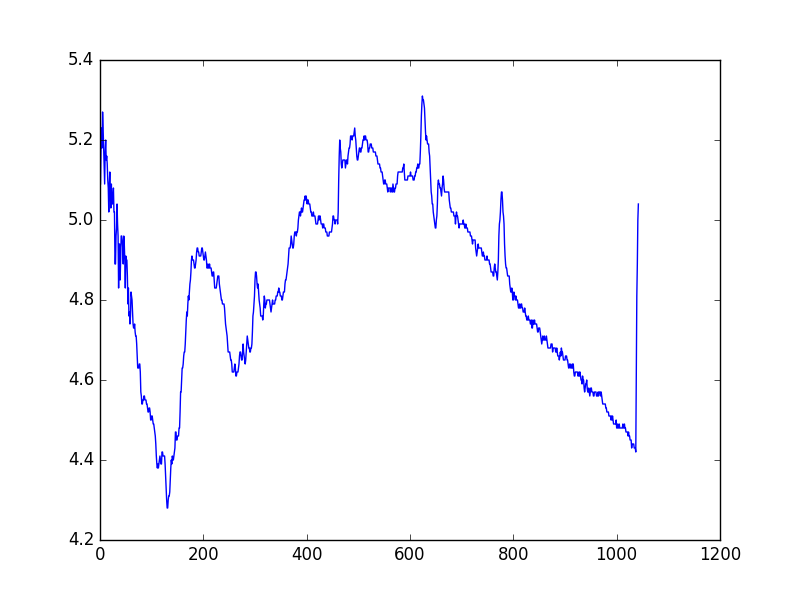
\includegraphics[width= \linewidth]{figures/ctd_figure12_1.pdf}

Finalmente, vamos plotar nosso gráfico incluindo uma linha horizontal
denotando a média dos valores. Calculamos a média usando o método mean
do Pandas.

\begin{Verbatim}[commandchars=\\\{\},frame=single,fontsize=\small, xleftmargin=0.5em]
\PY{n}{plt}\PY{o}{.}\PY{n}{plot}\PY{p}{(}\PY{n}{estacao1}\PY{p}{[}\PY{l+s+s1}{\PYZsq{}}\PY{l+s+s1}{Oxygen [ml l]}\PY{l+s+s1}{\PYZsq{}}\PY{p}{]}\PY{p}{)}
\PY{n}{plt}\PY{o}{.}\PY{n}{axhline}\PY{p}{(}\PY{n}{y}\PY{o}{=}\PY{n}{estacao1}\PY{p}{[}\PY{l+s+s1}{\PYZsq{}}\PY{l+s+s1}{Oxygen [ml l]}\PY{l+s+s1}{\PYZsq{}}\PY{p}{]}\PY{o}{.}\PY{n}{mean}\PY{p}{(}\PY{p}{)}\PY{p}{,} \PY{n}{linestyle} \PY{o}{=} \PY{l+s+s2}{\PYZdq{}}\PY{l+s+s2}{dashed}\PY{l+s+s2}{\PYZdq{}}\PY{p}{,}
\PY{n}{color} \PY{o}{=} \PY{l+s+s2}{\PYZdq{}}\PY{l+s+s2}{r}\PY{l+s+s2}{\PYZdq{}}\PY{p}{)}
\PY{n}{plt}\PY{o}{.}\PY{n}{title}\PY{p}{(}\PY{l+s+s2}{\PYZdq{}}\PY{l+s+s2}{Oxygen [ml l] for Station 1}\PY{l+s+s2}{\PYZdq{}}\PY{p}{)}
\PY{n}{plt}\PY{o}{.}\PY{n}{show}\PY{p}{(}\PY{p}{)}
\end{Verbatim}
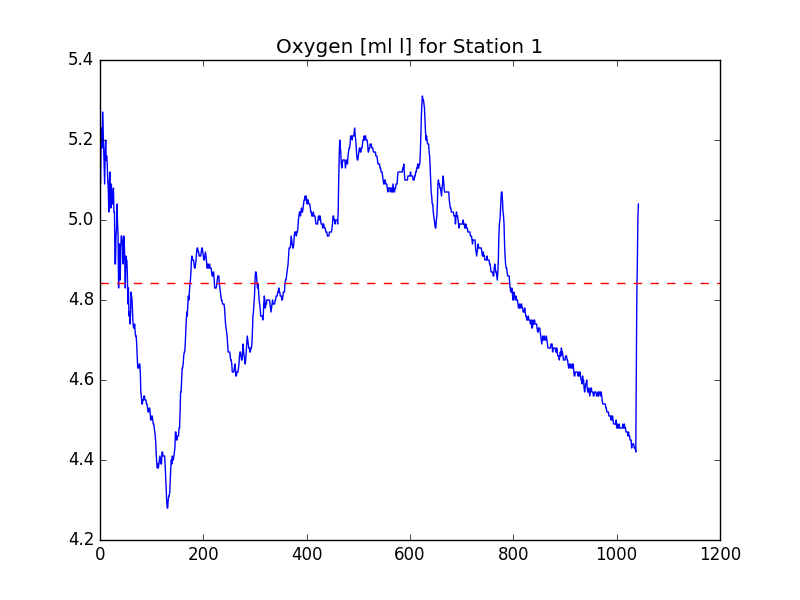
\includegraphics[width= \linewidth]{figures/ctd_figure13_1.pdf}
\end{document}